\chapter{SaaS, le teclologie che ne consentono la realizzazione}
Nel corso degli ultimi anni, con il proliferarsi delle piattaforme e dei servizi di Cloud Computing, sono nate e si sono sviluppate molte tecnologie per soddisfare le nuove esigenze e i nuovi requisiti appena visti che questa rivoluzione della fruizione del software ha comportato.

\section{Microservizi}
Un concetto fondamentale, di cui il Cloud Computing fa largamente uso, sono i mircoservizi. Cominciamo col darne una definizione abbastanza formale: "Lo stile architetturale a microservizi è un approccio allo sviluppo di una singola applicazione come insieme di piccoli servizi, ciascuno dei quali viene eseguito da un proprio processo e comunica con un meccanismo snello, spesso una HTTP API.(Martin Fowler)".

\paragraph{}
L'approccio è quello di dividere le funzionalità del sistema in più microservizi. Ad ogni microservizio corrisponde una necessità dell'utente. Una suddivisione modulare del sistema in base ai casi d'uso dell'utente è già presente da tempo nell'Object Oriented Design, ma la novità apportata dai microservizi è che il sistema con essi risulta scomposto in realtà in piccoli servizi completamente indipendenti tra loro. La comunicazione tra i servizi avviene attraverso la rete al fine di garantire l’indipendenza tra i servizi ed evitare ogni forma di accoppiamento. Ogni microservizio, infatti, rappresenta un'entità separata che generalmente viene pubblicata come un modulo di una Platform as a Service.

\subsection{Il modello monolitico a layer }
Secondo il classico modello a layer le funzionalità vengono suddivise in base al grado di astrazione tra i vari livelli, usando delle tecnologie proprie di ogni livello. Questi sono separati a livello logico e comunicano tra di loro. Con questa architettura però, nonostante ci sia questa suddivisione a strati, il software risulta essere un unico sistema monolitico, sebbene molti componenti possano essere comunque riusabili.

\begin{figure}[h!]
	\centering
	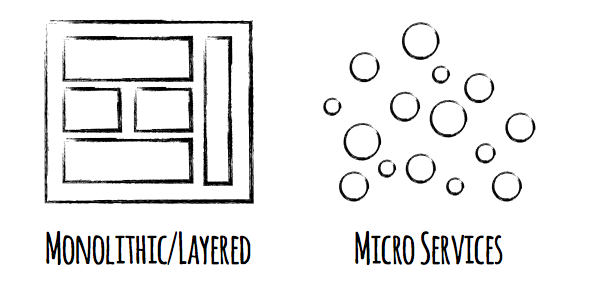
\includegraphics[width=\textwidth,keepaspectratio=true]{capitoli/imgs/disegnoMicrosMonol.png}
	\caption{Il modello monolitico e i microservizi}
\end{figure}

\subsection{Confronto tra l'architettura a microservizi e il modello monolitico}
La scelta di adottare uno o l'altro approccio viene dopo un'attenta analisi dei requisiti che il sistema deve soddisfare. In questo studio però va anche tenuto conto quanto le esigenze possano cambiare nei futuri utilizzi del software.
\begin{itemize}
	\item La struttura interna di tutto un sistema monolitico è composta principalmente dai layer di interfacciamento con l'utente, logica di business e persistenza dei dati. In un'architettura a microservizi non troviamo questa divisione a livello di sistema, ma la ritroviamo semmai all'interno di un singolo microservizio atomico. Ogni microservizio, ad esempio, si occuperà di preservare il suo stato tramite l'utilizzo di un proprio database non condiviso con gli altri microservizi. 
	
	\item Uno dei fattori chiave da considerare è la scalabilità. Per scalare un'applicazione monolitica occorre necessariamente clonarla in più server, macchine virtuali o contenitori.
	
	\item Quando occorre scalare orizzontalmente un'architettura a microservizi, si creano e si distribuiscono indipendentemente tra loro repliche dei microservizi in più server o container. 
\end{itemize}


\begin{figure}[h!]
	\centering
	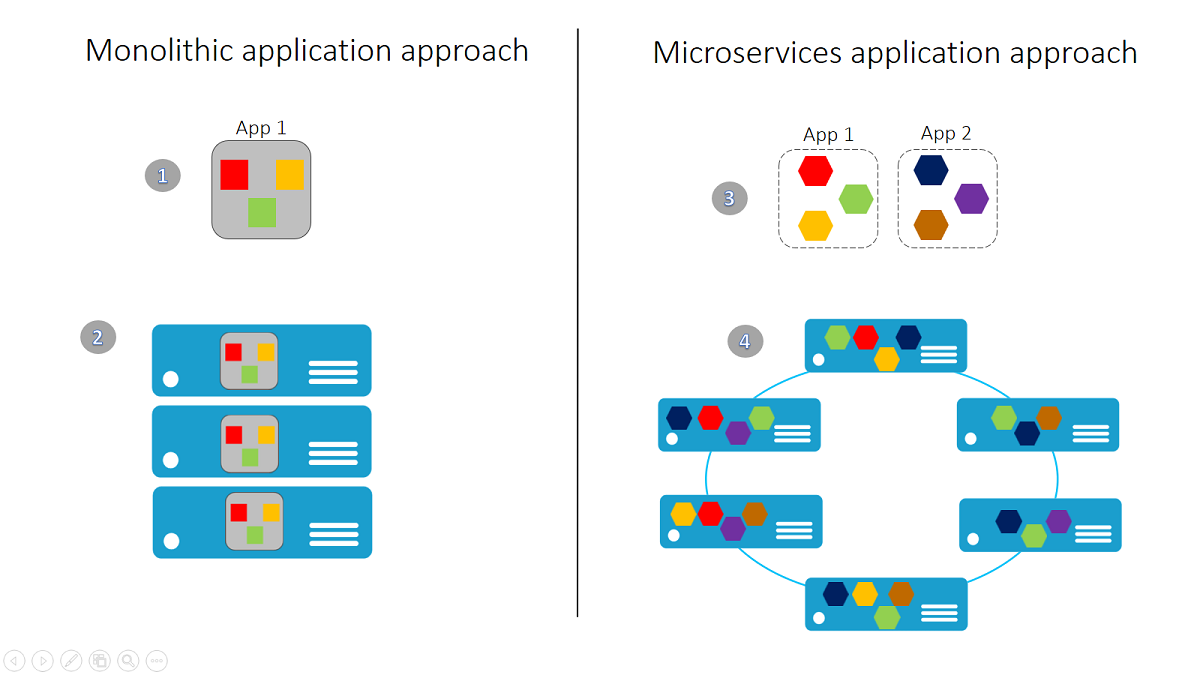
\includegraphics[width=\textwidth,keepaspectratio=true]{capitoli/imgs/monosvmicro.png}
	\caption{Il modello monolitico e i microservizi}
\end{figure}

\subsection{Vantaggi e svantaggi di un'architettura a microservizi}
Un'architettura di questo tipo porta con se ovviamente anche i suoi svantaggi e i suoi vantaggi. Sono proprio questi ultimi che la rendono molto adatta al Cloud Computing.

\subsubsection{Vantaggi}
\begin{itemize}
	\item  Velocità \\
	L'architettura a microservizi è quella che si sposa meglio con la metodologia agile. Lo sviluppo di un microservizio dovrebbe avere una durata di circa due settimane e ciò spinge molto ad avere fin da subito piccole porzioni del sistema (i servizi appunto), pronte, testabili ed utilizzabili. Ogni microservizio inoltre è autonomo e può quindi giungere in ambiente di produzione indipendentemente dagli altri, reagendo molto velocemente alle esigenze di mercato.
\end{itemize}